\documentclass{report}
\usepackage{graphicx} % Required for inserting images
\usepackage{amsmath}
\usepackage{hyperref}

\title{DS250 (DAV) Class Module}
\author{DR.GAGAN RAJ GUPTA} 
\date{January 2025}

\begin{document}

\maketitle

\section{Introduction}

 Notes on Plotting Histograms and Heatmaps 
 \setlength{\parskip}{1em}

 

1. \textbf{HISTOGRAMS}:-


\setlength{\parskip}{1em}


 
A histogram is a graphical representation of the distribution of data. It divides the entire range of values into intervals (called bins) and counts the number of data points that fall into each bin.


\textit\setlength{\parindent}{} 
\textit{{Mathematical Definition}:-} 


Let  be the data points. Divide the range of data into  bins, where:

The bin width  is:

w = \frac{\text{max}(x) - \text{min}(x)}{k}

b_i \leq x < b_{i+1} 

Here,  and  are the edges of the -th bin.


\textit{Steps to Plot a Histogram:-}


1. Choose the number of bins: Use the rule of thumb or algorithms like the Sturges' formula:



k = \lceil \log_2(n) + 1 \rceil

2. Plot the frequencies using bar heights.


\setlength{\parskip}{1em}


Python Code Example:-


import matplotlib.pyplot as plt

import numpy as np


% Sample data

data = np.random.normal(0, 1, 1000)

% Plotting the histogram

plt.hist(data, bins=30, edgecolor='black', alpha=0.7)

plt.title('Histogram')

plt.xlabel('Value')

plt.ylabel('Frequency')

plt.show()


\setlength{\parskip}{1em}

\textit{ACTIVITY ON HISTOGRAM:- }

\subsection{Part A: Word Length Histogram}
\subsubsection*{Objective}
Create a histogram that represents the frequency of words based on their length in any paragraph from your preferred book.

\subsubsection*{Steps}
\begin{enumerate}
    \item Choose a paragraph from your favorite book.
    \item Count the number of letters in each word.
    \item Group words by their lengths (e.g., words with 1 letter, 2 letters, etc.).
    \item Plot the histogram with:
    \begin{itemize}
        \item \textbf{X-axis}: Word lengths.
        \item \textbf{Y-axis}: Frequency of words of each length.
    \end{itemize}
\end{enumerate} 

\subsection{Part B: Starting Letter Histogram}
\subsubsection*{Objective}
Create a histogram to analyze the frequency of words starting with each letter of the alphabet.

\subsubsection*{Steps}
\begin{enumerate}
    \item Use the same paragraph as in Part A.
    \item Count how many words start with each letter (A-Z).
    \item Plot the histogram with:
    \begin{itemize}
        \item \textbf{X-axis}: Starting letters (A-Z).
        \item \textbf{Y-axis}: Frequency of words starting with each letter.
    \end{itemize}
\end{enumerate}

\begin{figure}
    \centering
    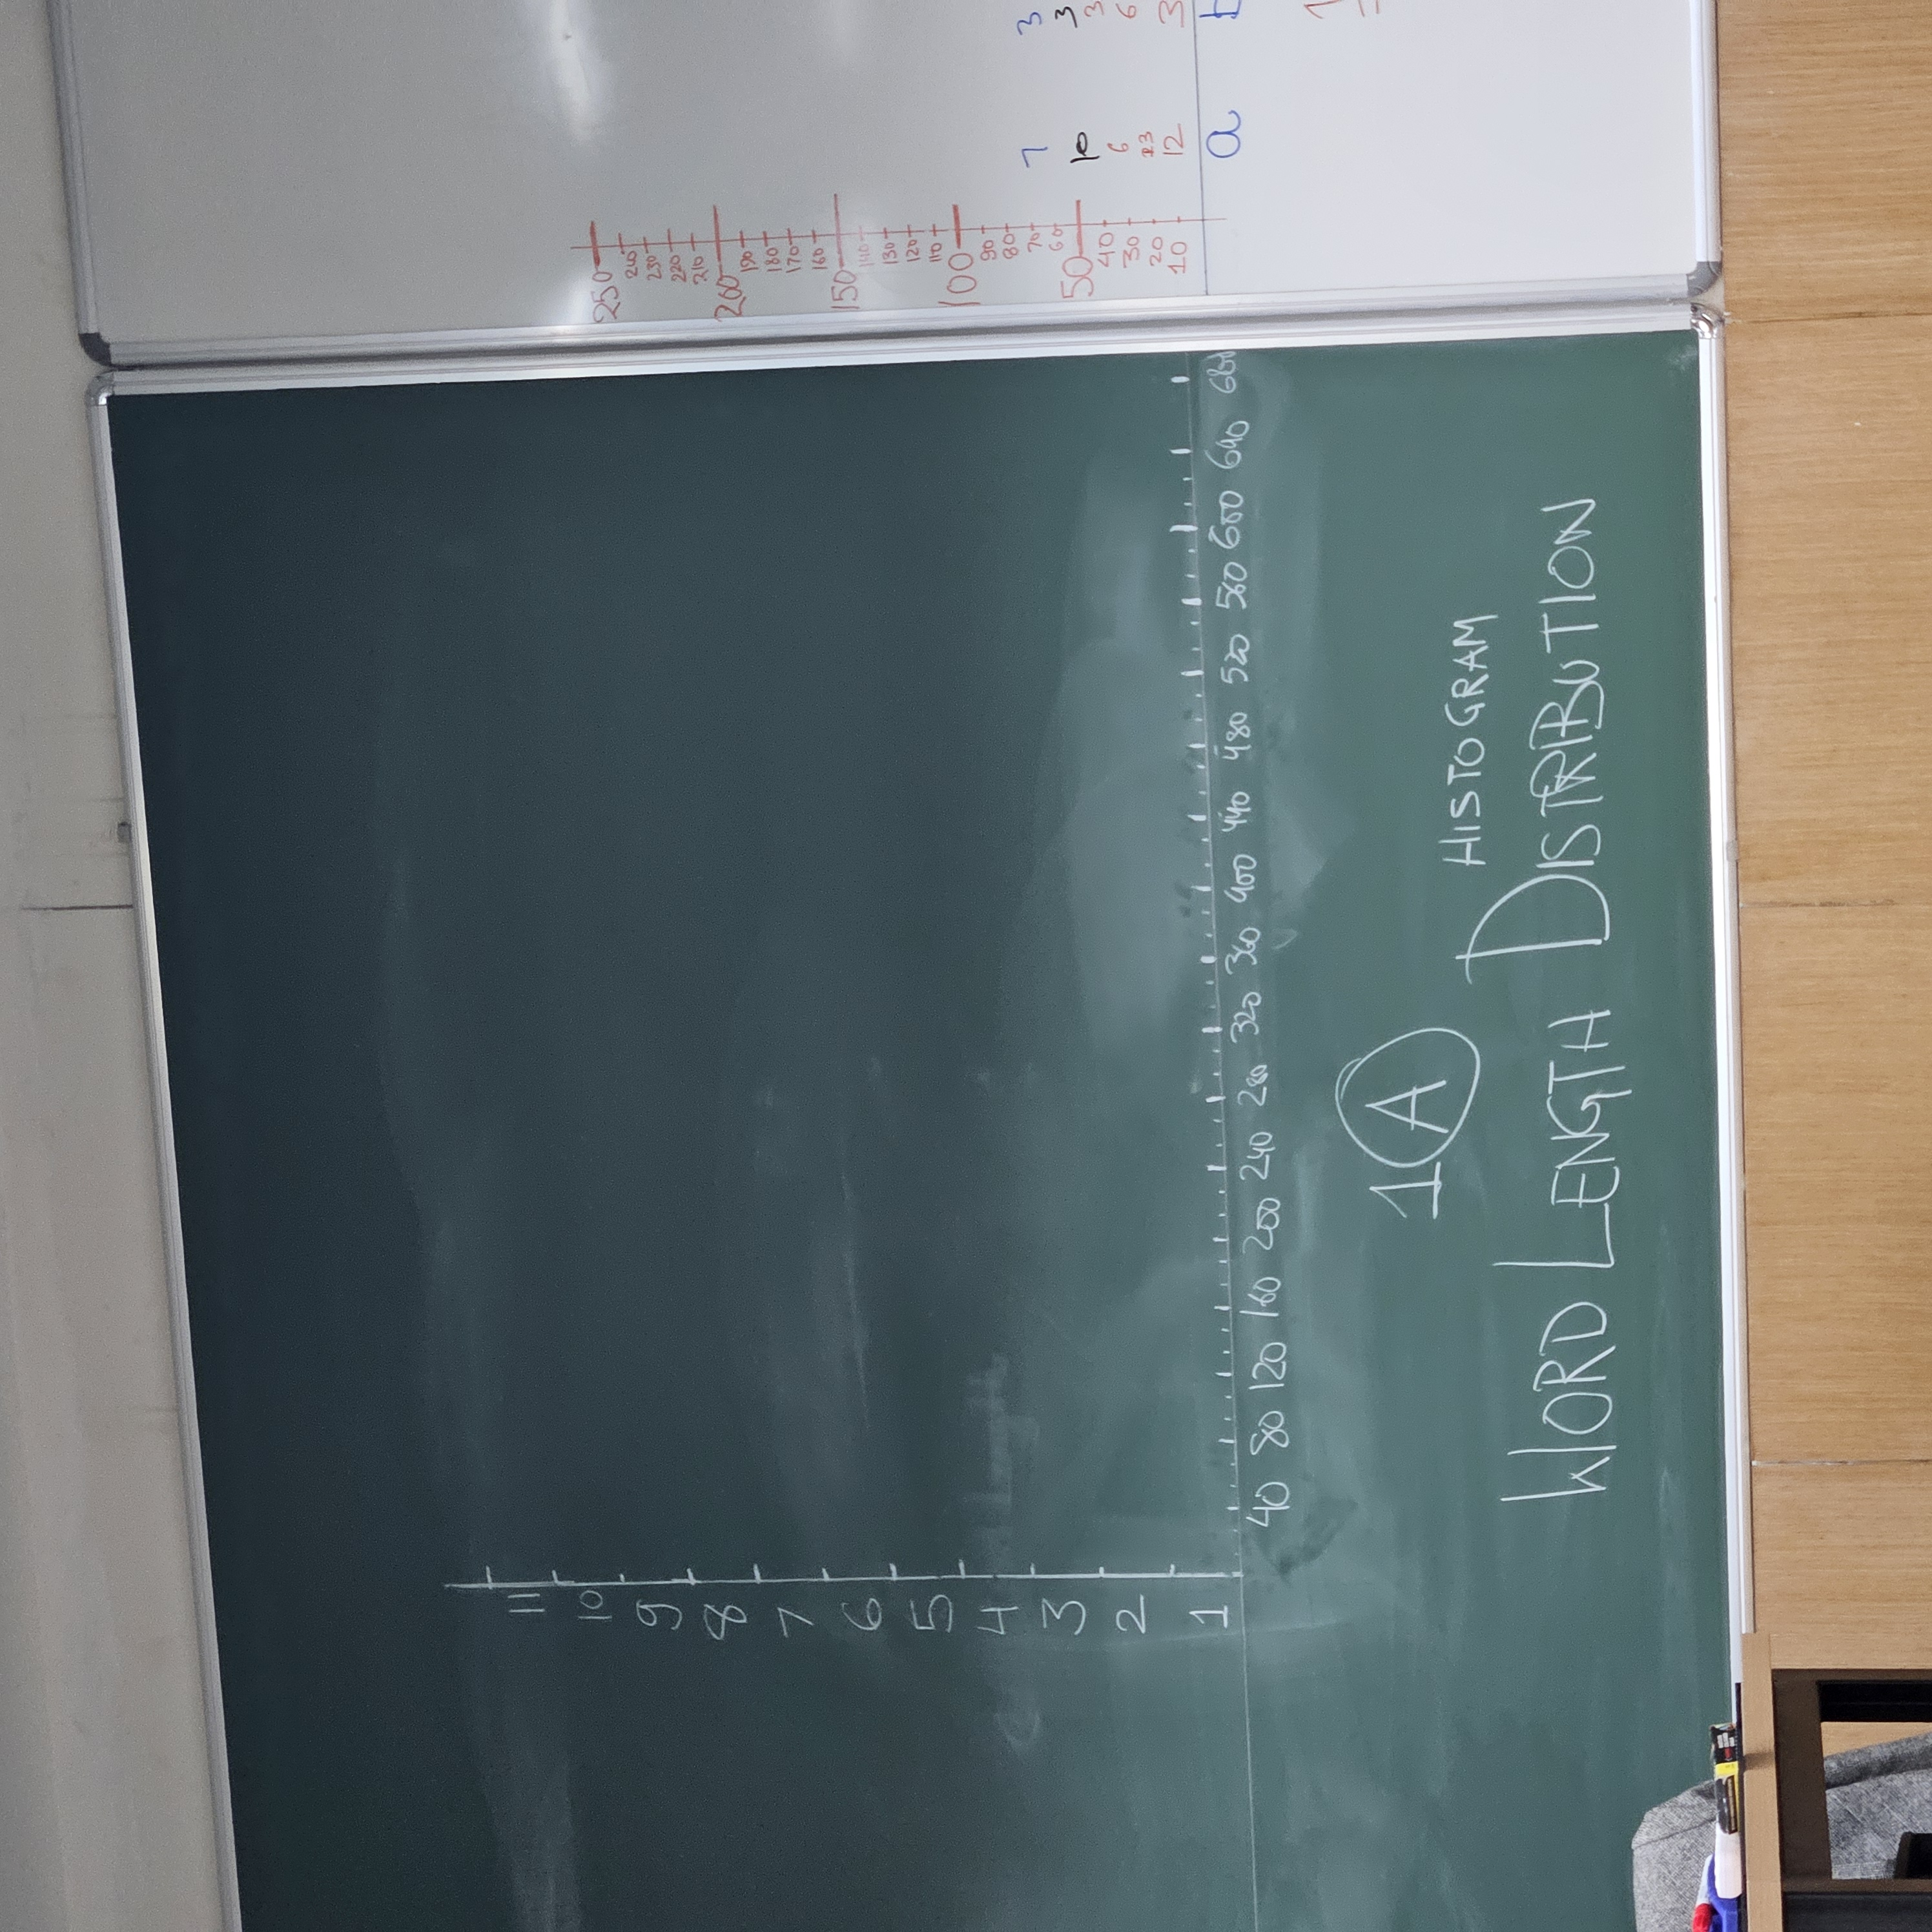
\includegraphics[width=0.6\linewidth , angle=270]{word length.jpg}
    \caption{word length distribution}
    \label{fig:word length}
\end{figure}

\begin{figure}
    \centering
    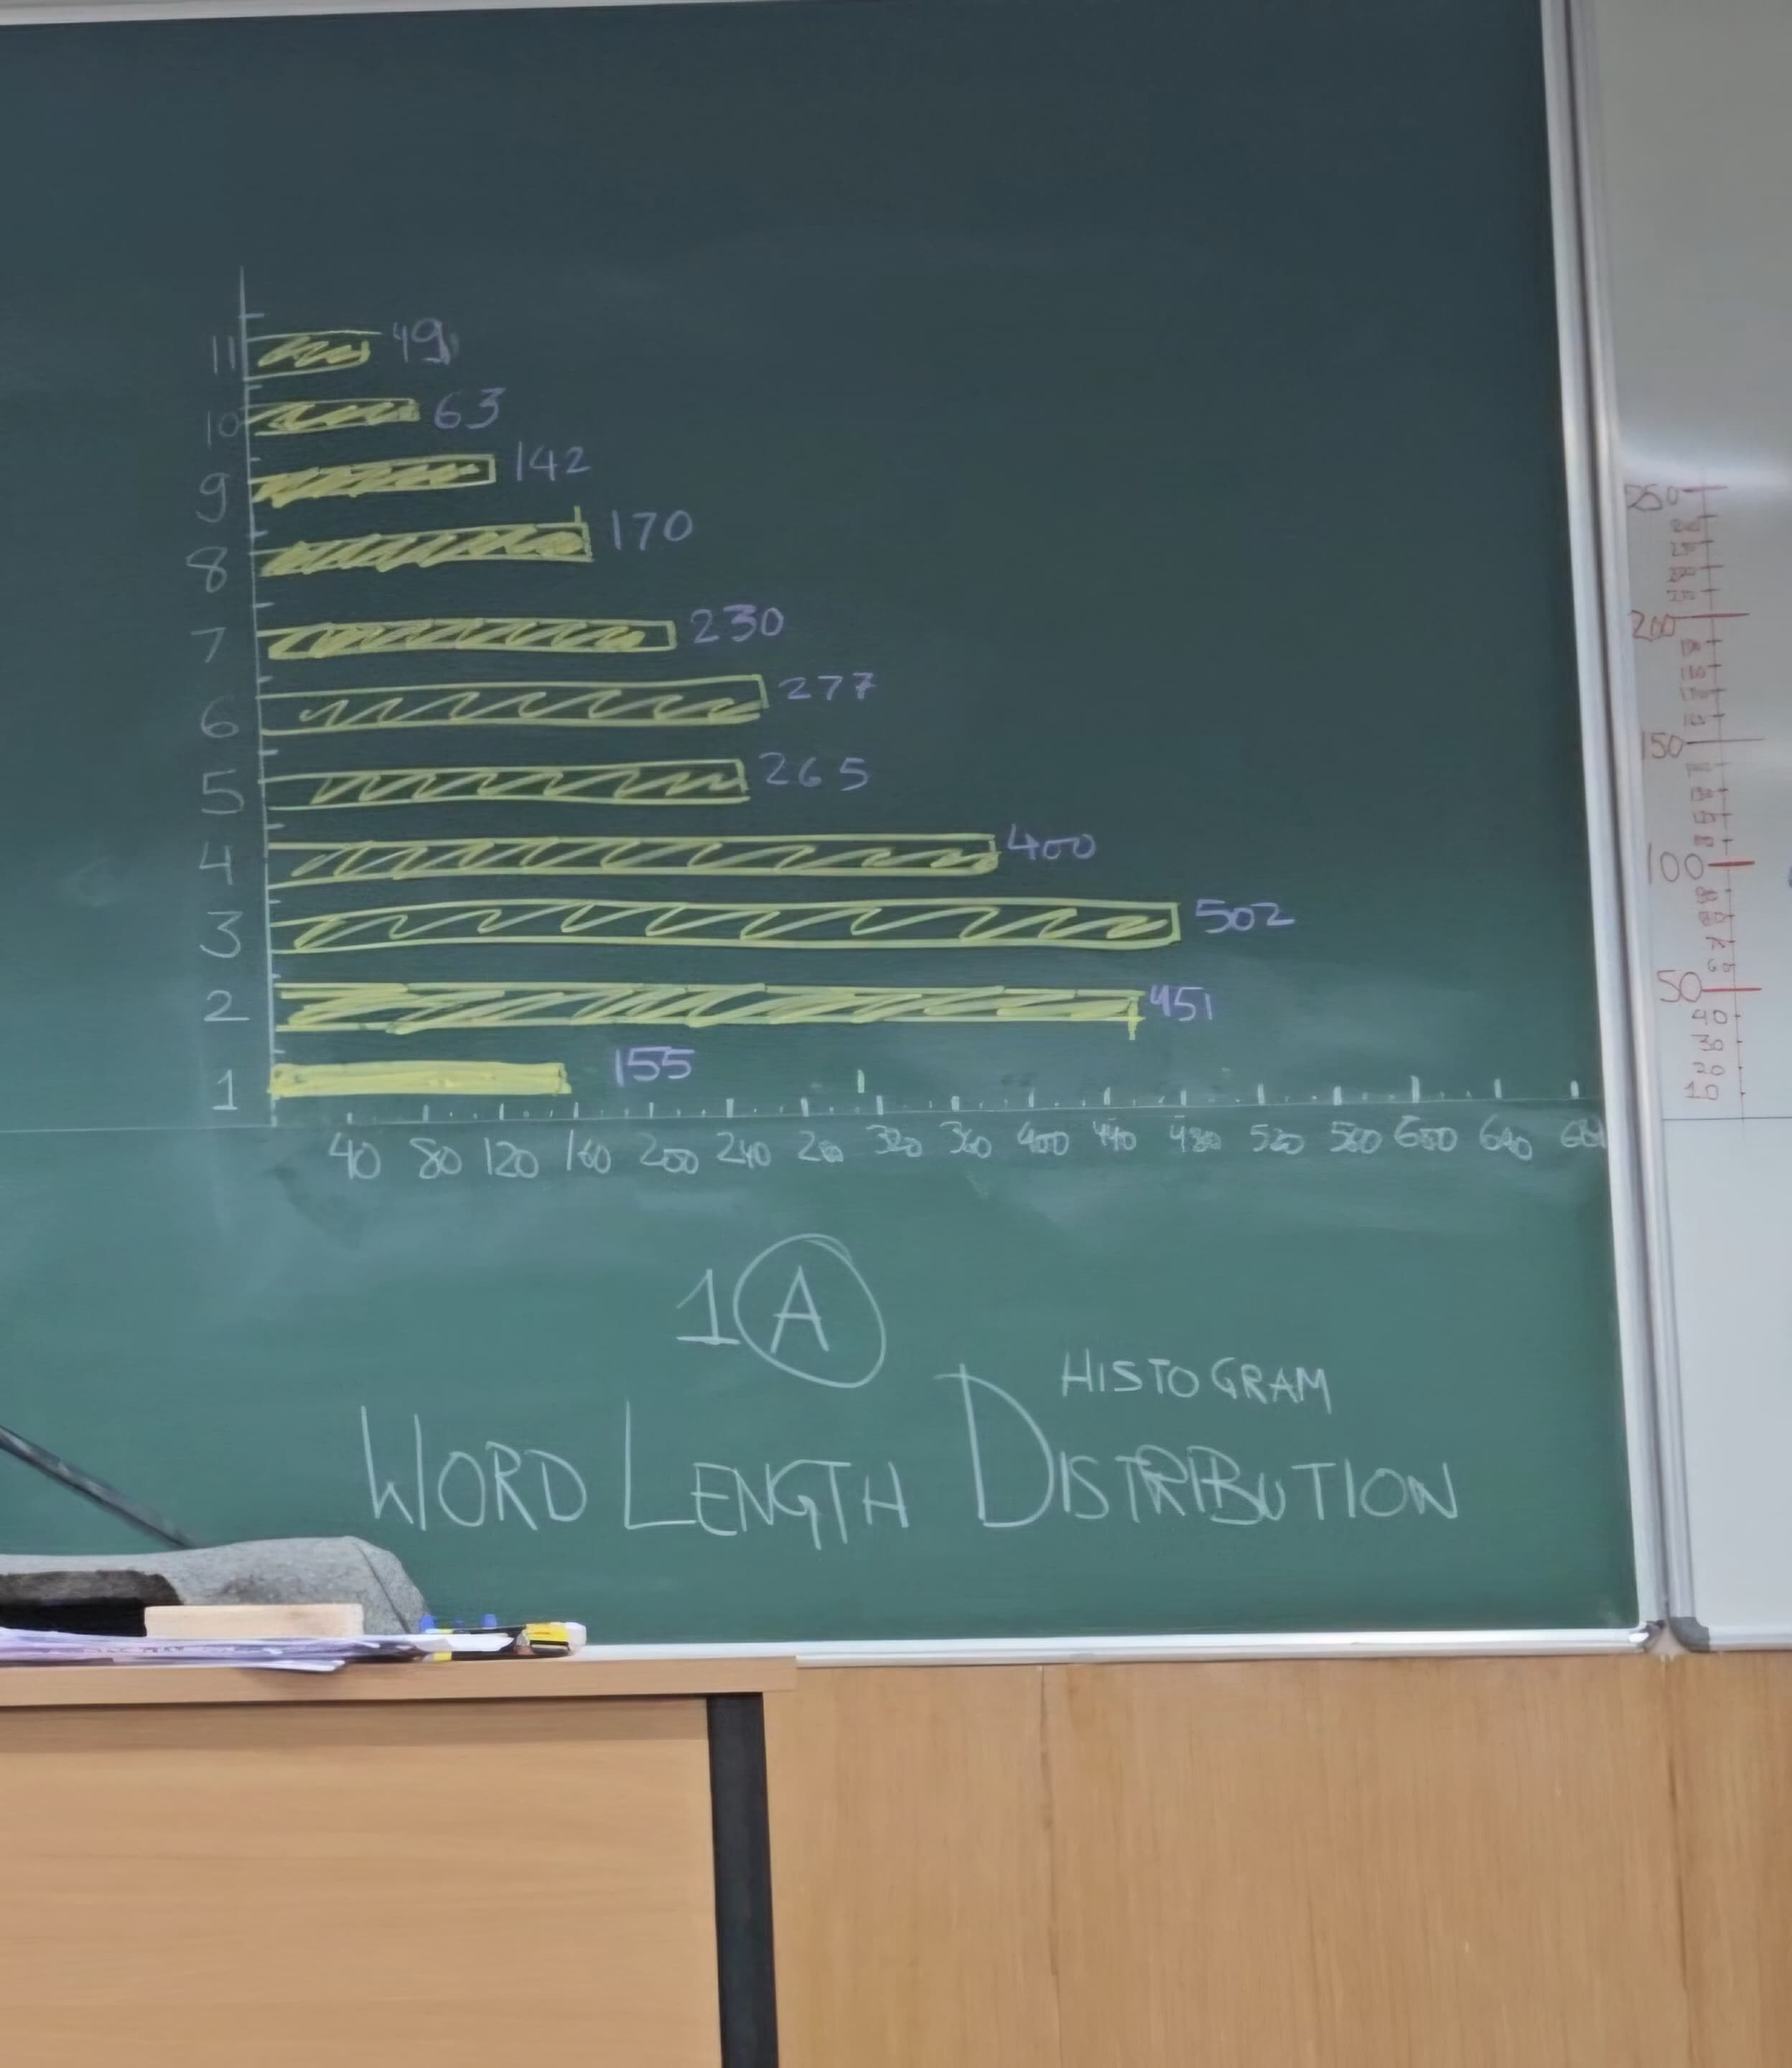
\includegraphics[width=0.7\linewidth]{word_length Distribution.jpeg}
    \caption{Word length Distribution}
    \label{fig:word length}
\end{figure}


\subsection{Part C: Forecasting with Weight and Height Functions}
\subsubsection*{Objective}
Plot histograms using functions for weight and height over time.

\subsubsection*{Functions}
Define the following functions:
\begin{align*}
    w(t) &= t + 2, \quad \text{(Weight function)} \\
    h(t) &= 3t + 5, \quad \text{(Height function)}
\end{align*}
where \( t \) represents time (from the beginning to today).

\subsubsection*{Steps}
\begin{enumerate}
    \item Create data points for different values of \( t \) (e.g., \( t = 0, 1, 2, \dots \)).
    \item Calculate \( w(t) \) and \( h(t) \) for each \( t \).
    \item Plot the histogram using:
    \begin{itemize}
        \item \textbf{X-axis}: Time (\( t \)).
        \item \textbf{Y-axis}: Weight (\( w(t) \)) or Height (\( h(t) \)).
    \end{itemize}
\end{enumerate} 

\begin{figure}
    \centering
    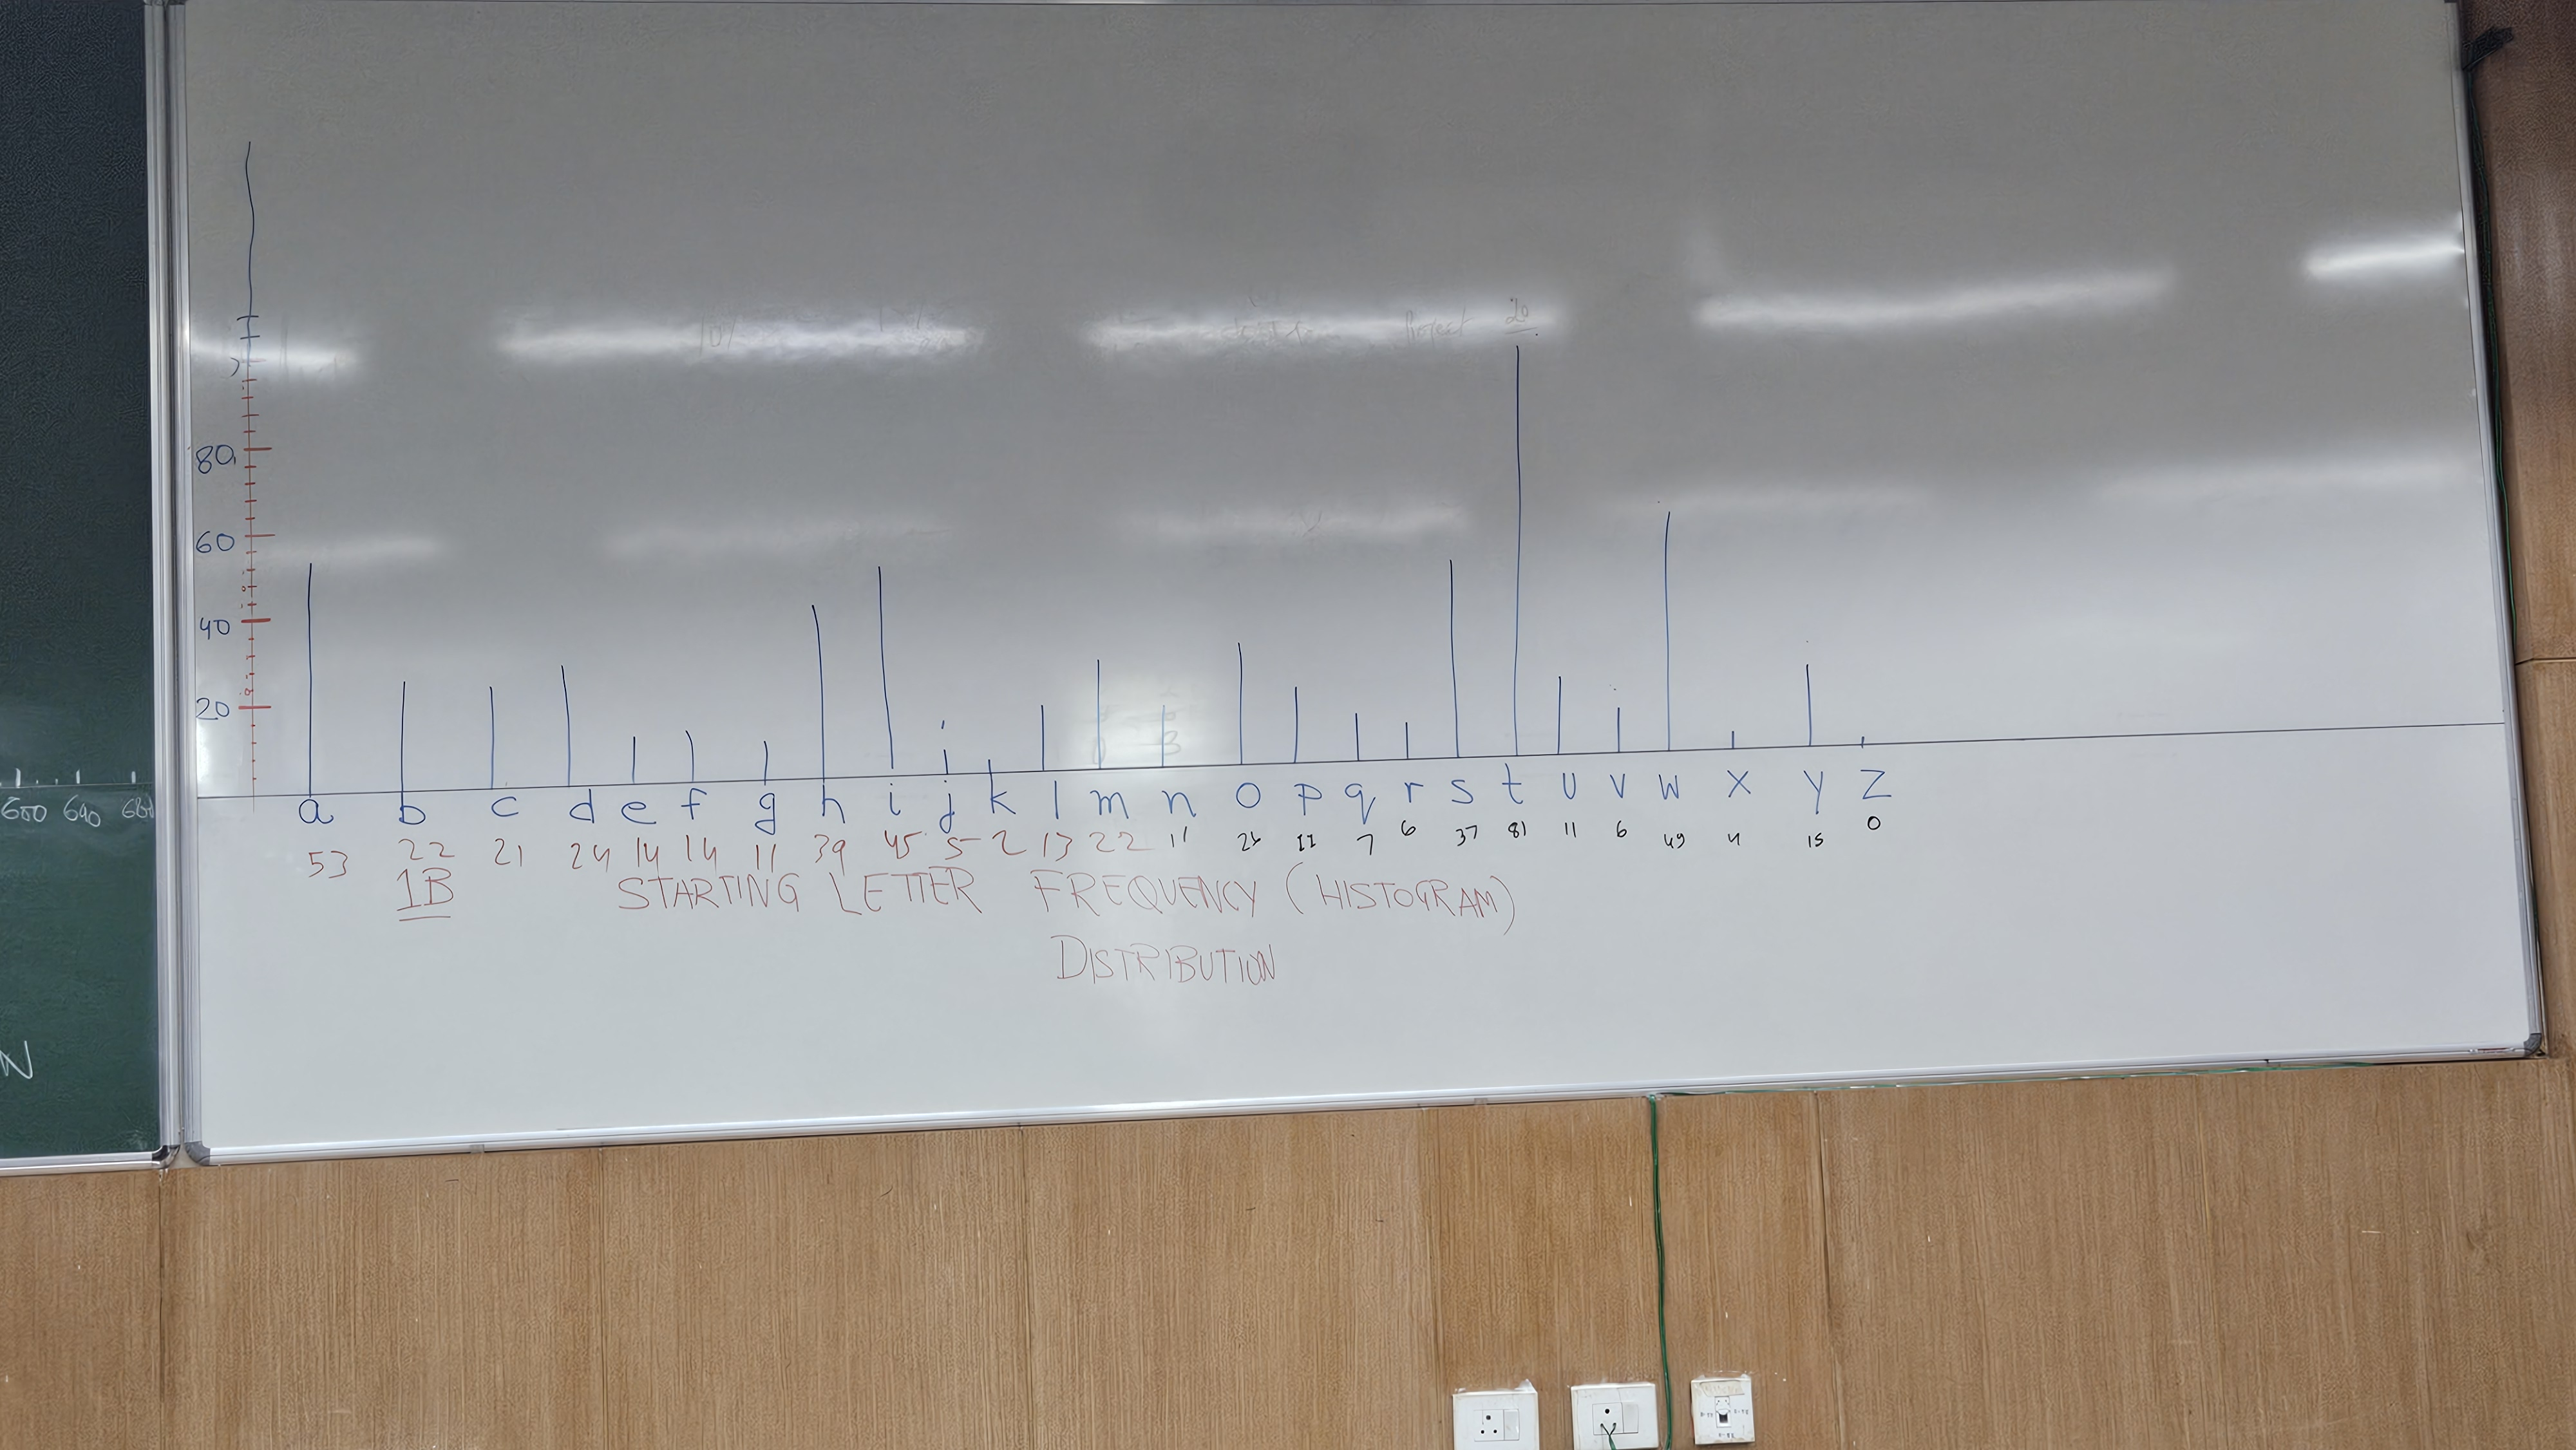
\includegraphics[width=0.8\linewidth]{starting_letter_frequency.jpg}
    \caption{Starting letter distribution}
    \label{fig:starting_letter_distribution}
\end{figure} 


\textbf{Click here to watch the video:} \href{https://drive.google.com/file/d/1g_NWFWEwnrwKtEe_6Ub3wr88oSFAZrdw/view?usp=drive_link}{Watch Video}



\textit{ANSWER THE FOLLOWING QUESTIONS}

Q1. A. PLot the histogram on the basis of word length of any Paragraph of your preferred book.


B. PLot the Starting letter of the Word.


C. Use the following function to PLot the same:- 


    Weight = w(t),
    Height = h(t)
     where :-
     
     time = t (begining, ..................., Today)

     forecast the following in Histogram Plotting.


D. Plot a histogram for the dataset [1, 2, 2, 3, 3, 3, 4, 4, 4, 4] with customizations:

Change color, labels, and title.

Add gridlines and annotate the highest frequency bin.

E. Import a real-world dataset (e.g., Iris dataset).

Plot histograms for numerical columns like petal length or sepal width.
     
     



---

\setlength{\parskip}{1em}




\ 
\ 
\ 
\ 

2. \textbf{HEAT MAPS}



A heatmap is a data visualization technique used to represent data in a
matrix format with varying intensities of color to show magnitude.


Mathematical Definition:-


For a matrix  with elements , a heatmap assigns a color  to each cell based on a colormap :


c_{ij} = C(a_{ij})

\textit{Steps to Create a Heatmap:-}


1. Normalize the data: Rescale values if needed.


2. Choose a colormap: Maps numerical values to colors.


3. Visualize the data as a grid.


\setlength{\parskip}{1em}



\textbf{Python Code Example:-}


import seaborn as sns

import numpy as np

import matplotlib.pyplot as plt


%Sample data

data = np.random.rand(10, 10)

%Plotting the heatmap

sns.heatmap(data, annot=True, cmap='viridis')

plt.title('Heatmap')





\setlength{\parskip}{1em}



Part 1: \textbf{Basics of Vector Algebra}

\setlength{\parskip}{1em}

 1.1 \textbf{Vectors}


A vector is a quantity that has both magnitude and direction. It can be represented in the Cartesian coordinate system with components along the x, y, and z axes. 

For example, a vector \(\vec{A}\) in two-dimensional space can be written as:

\[
\vec{A} = A_x \hat{i} + A_y \hat{j}
\]

where:
- \( A_x \) and \( A_y \) are the components of the vector along the x and y axes, respectively.
- \(\hat{i}\) and \(\hat{j}\) are the unit vectors along the x and y axes.


\setlength{\parskip}{1em}


1.2 \textbf{Vector Operations}:-



*Addition of Vectors*: The sum of two vectors is obtained by adding their corresponding components.

\[
\vec{A} + \vec{B} = (A_x + B_x) \hat{i} + (A_y + B_y) \hat{j}
\]

*Scalar Multiplication*: When a vector is multiplied by a scalar, each component of the vector is multiplied by that scalar.

\[
k \cdot \vec{A} = k \cdot A_x \hat{i} + k \cdot A_y \hat{j}
\]

*Dot Product*: The dot product of two vectors is a scalar quantity given by:

\[
\vec{A} \cdot \vec{B} = A_x \cdot B_x + A_y \cdot B_y
\]

*Cross Product*: The cross product of two vectors gives a vector perpendicular to both vectors. For two 2D vectors \(\vec{A} = A_x \hat{i} + A_y \hat{j}\) and \(\vec{B} = B_x \hat{i} + B_y \hat{j}\), the cross product is:

\[
\vec{A} \times \vec{B} = (A_x B_y - A_y B_x) \hat{k}
\]

where \(\hat{k}\) is the unit vector along the z-axis.

\begin{figure}
    \centering
    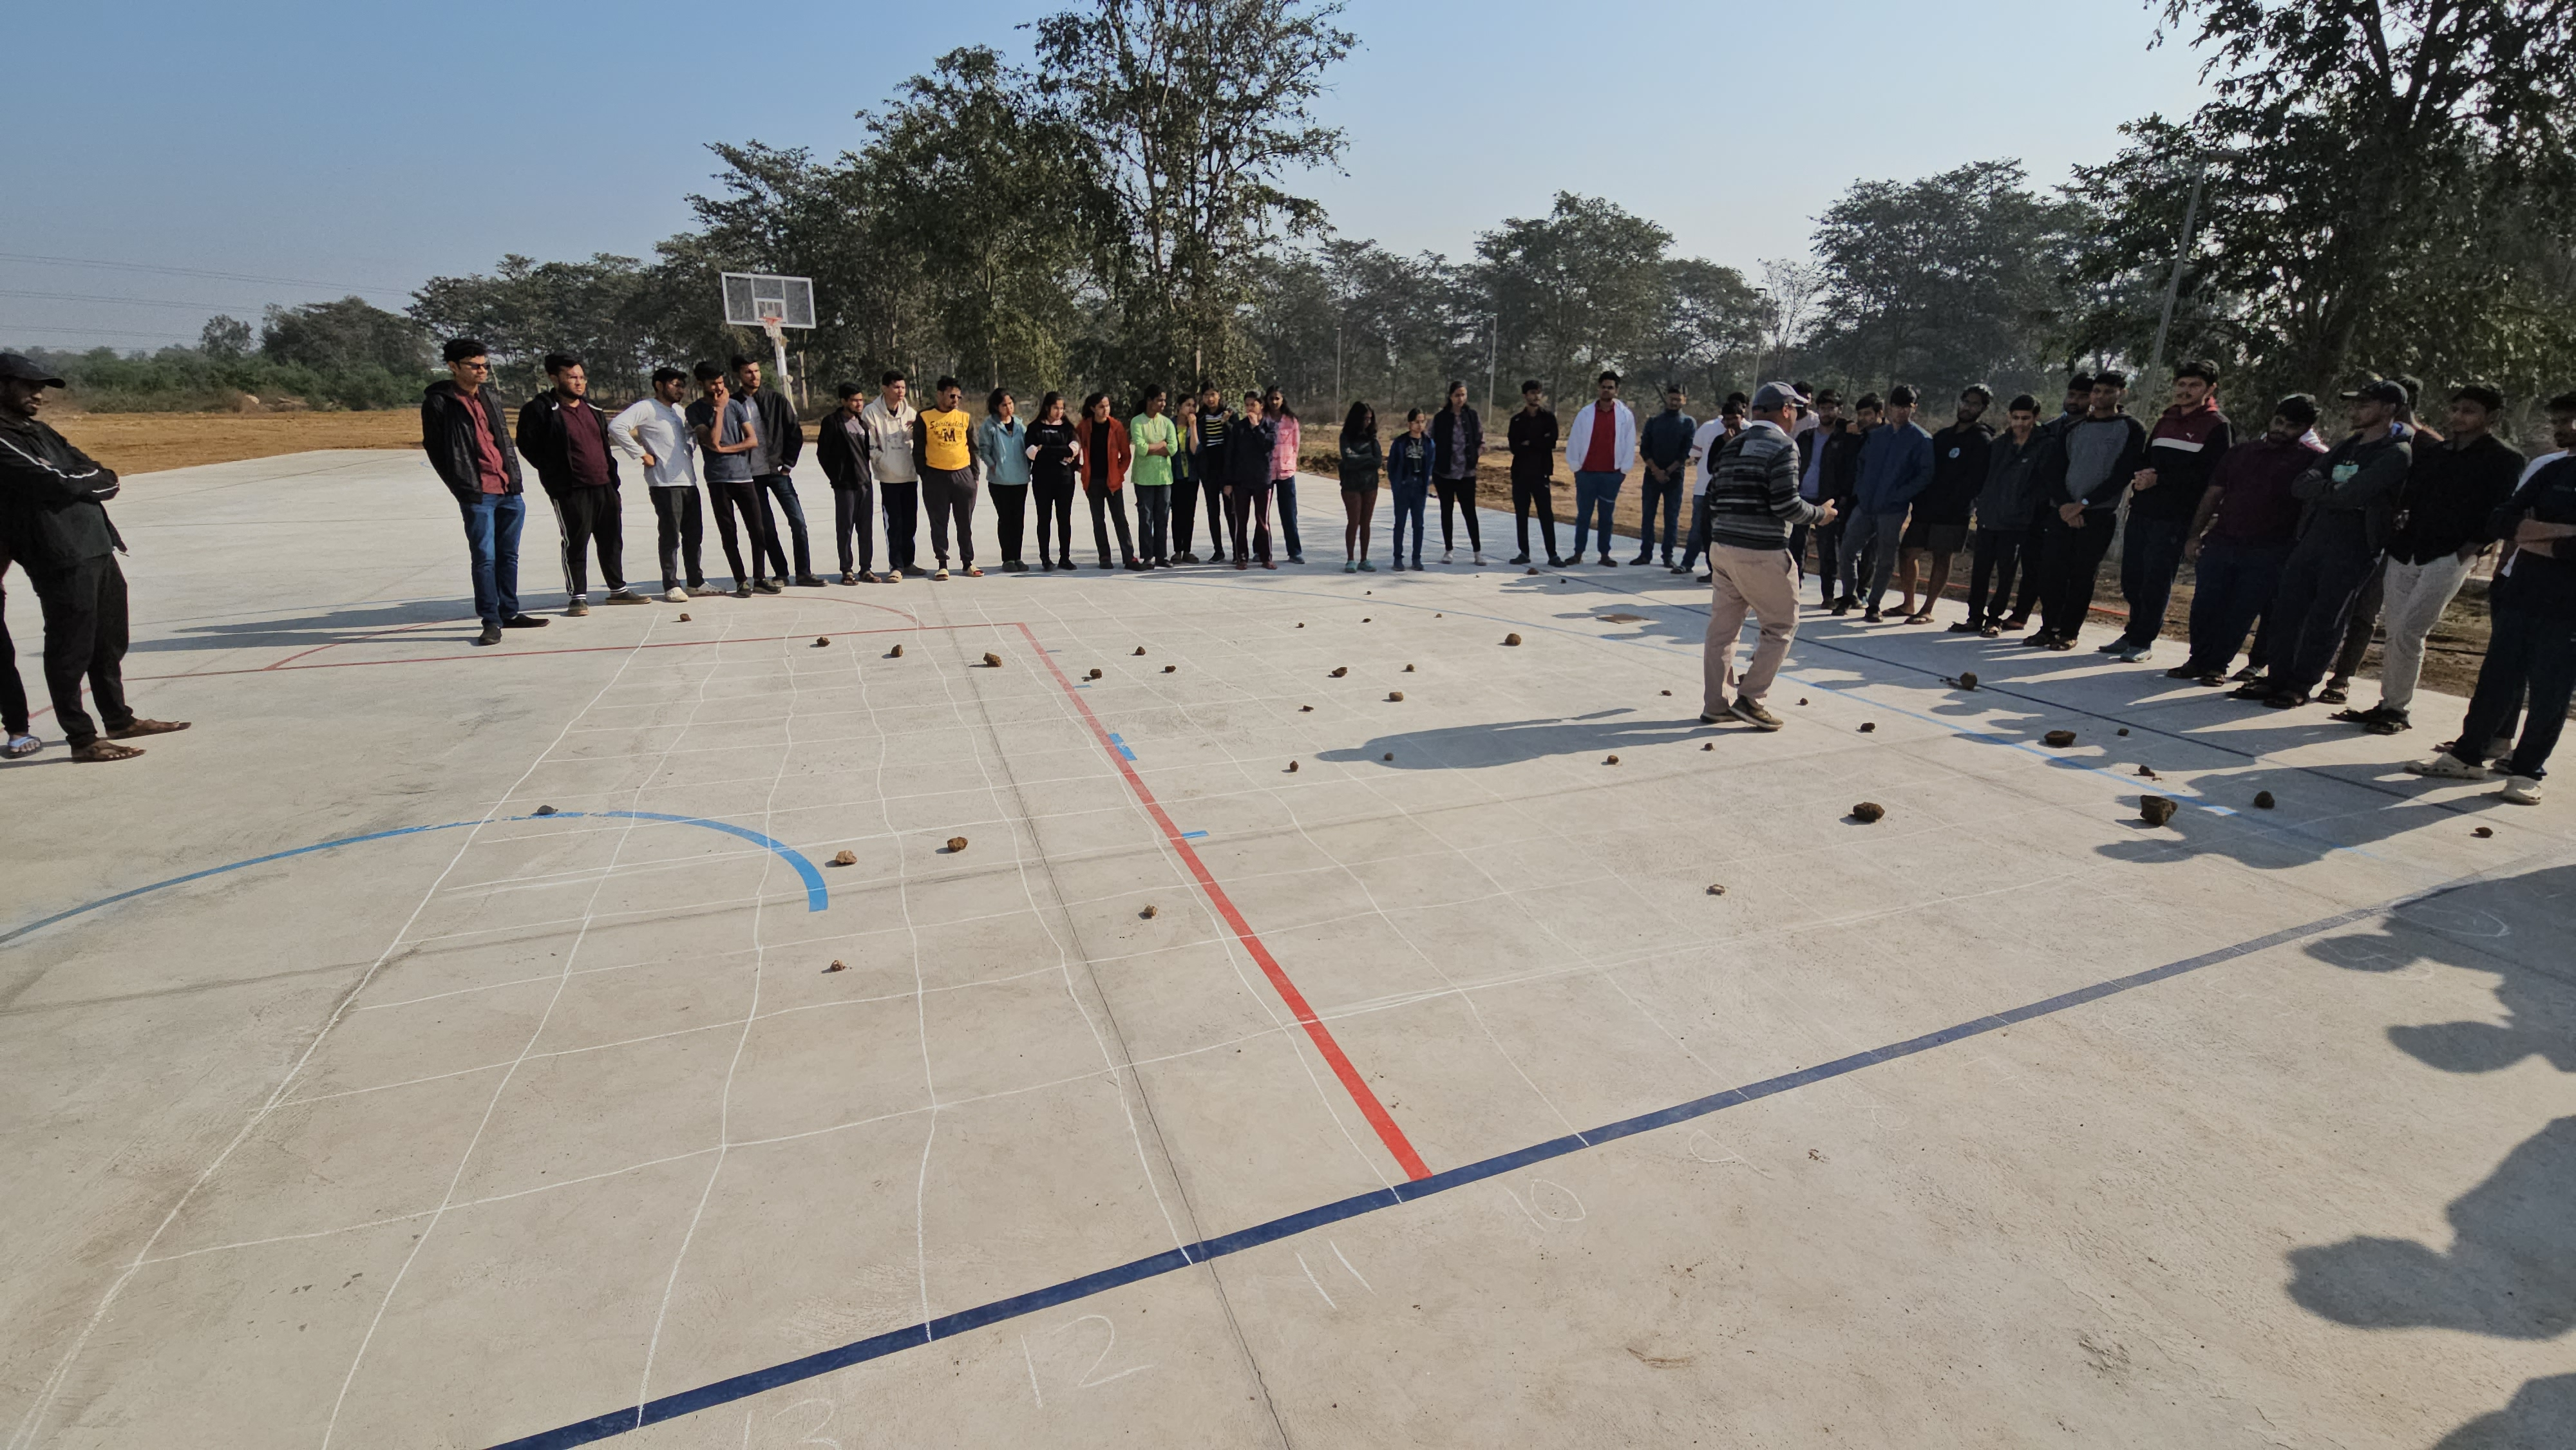
\includegraphics[width=0.7\linewidth]{vector matrix.jpg}
    \caption{VECTOR MATRIX}
    \label{fig:VECTOR MATRIX}
\end{figure}


---
### Part 2: \textbf{Tug of War Problem}


In this problem, we will model a tug of war scenario where three people are pulling a rope from different directions. The goal is to determine the resulting force on the rope by calculating the Vector that is  sum of all the individual forces.

#### \textbf{2.1 Problem Description}

\setlength{\parskip}{1em}

Three people are pulling on a rope from different directions:
\setlength{\parskip}{1em}

- Person 1 applies a force of \( \vec{F}_1 = 10 \hat{i} + 5 \hat{j} \) Newtons.\ 

- Person 2 applies a force of \( \vec{F}_2 = -8 \hat{i} + 7 \hat{j} \) Newtons.\ 

- Person 3 applies a force of \( \vec{F}_3 = 3 \hat{i} - 6 \hat{j} \) Newtons.

We will calculate the net force on the rope by adding these vectors together and analyze the direction and magnitude of the result.

\setlength{\parskip}{1em}

2.2 \textit{Steps to solve:-}

1. Add the vectors \( \vec{F}_1, \vec{F}_2, \) and \( \vec{F}_3 \).\ 

2. Compute the magnitude of the resulting vector. \ 

3. Analyze the direction of the resultant vector.


\setlength{\parskip}{1em}
\ 
\ 


\textbf{ACTIVITY}:-


\subsection{Activity: Understanding Vectors through Tug of War}
\subsubsection*{Objective}
The goal of this activity is to understand the concept of vectors, their operations (addition, magnitude, and direction), by modeling a tug of war scenario where three people are pulling a rope from different directions.

\subsubsection*{Problem Description}
Three people are pulling on a rope from different directions:
\begin{itemize}
    \item Person 1 applies a force of \( \vec{F}_1 = 10 \hat{i} + 5 \hat{j} \) Newtons.
    \item Person 2 applies a force of \( \vec{F}_2 = -8 \hat{i} + 7 \hat{j} \) Newtons.
    \item Person 3 applies a force of \( \vec{F}_3 = 3 \hat{i} - 6 \hat{j} \) Newtons.
\end{itemize}

We will determine the net force on the rope by calculating the vector sum of \( \vec{F}_1, \vec{F}_2, \) and \( \vec{F}_3 \). Additionally, we will compute the magnitude and analyze the direction of the resultant vector.

\subsubsection*{Steps to Solve}
\begin{enumerate}
    \item Add the vectors \( \vec{F}_1, \vec{F}_2, \) and \( \vec{F}_3 \):
    \begin{align*}
        \vec{F}_{\text{net}} &= \vec{F}_1 + \vec{F}_2 + \vec{F}_3 \\
        &= (10 \hat{i} + 5 \hat{j}) + (-8 \hat{i} + 7 \hat{j}) + (3 \hat{i} - 6 \hat{j}) \\
        &= (10 - 8 + 3) \hat{i} + (5 + 7 - 6) \hat{j} \\
        &= 5 \hat{i} + 6 \hat{j}.
    \end{align*}

    \item Compute the magnitude of the resulting vector \( \vec{F}_{\text{net}} \):
    \begin{align*}
        |\vec{F}_{\text{net}}| &= \sqrt{(5)^2 + (6)^2} \\
        &= \sqrt{25 + 36} \\
        &= \sqrt{61} \approx 7.81 \, \text{N}.
    \end{align*}

    \item Analyze the direction of the resultant vector:
    \begin{align*}
        \theta &= \tan^{-1} \left( \frac{\text{Vertical component}}{\text{Horizontal component}} \right) \\
        &= \tan^{-1} \left( \frac{6}{5} \right) \\
        &= \tan^{-1} (1.2) \\
        &\approx 50.19^\circ \, \text{above the positive } \hat{i} \text{-axis}.
    \end{align*}
\end{enumerate}

\subsubsection*{Discussion Points}
\begin{itemize}
    \item \textbf{Addition of Vectors:} Demonstrates how forces combine in two dimensions.
    \item \textbf{Magnitude of the Resultant Vector:} Shows how to calculate the strength of the net force.
    \item \textbf{Direction of the Resultant Vector:} Explains the use of trigonometry to find the orientation of the net force.
\end{itemize}

\subsubsection*{Extension Activity}
Challenge students to:
\begin{itemize}
    \item Add more participants with different forces and calculate the new net force.
    \item Use graphical methods (parallelogram or head-to-tail) to verify the calculations.
    \item Explore real-world scenarios where vectors play a role, such as forces in sports or physics problems involving motion.
\end{itemize}

\begin{figure}
    \centering
    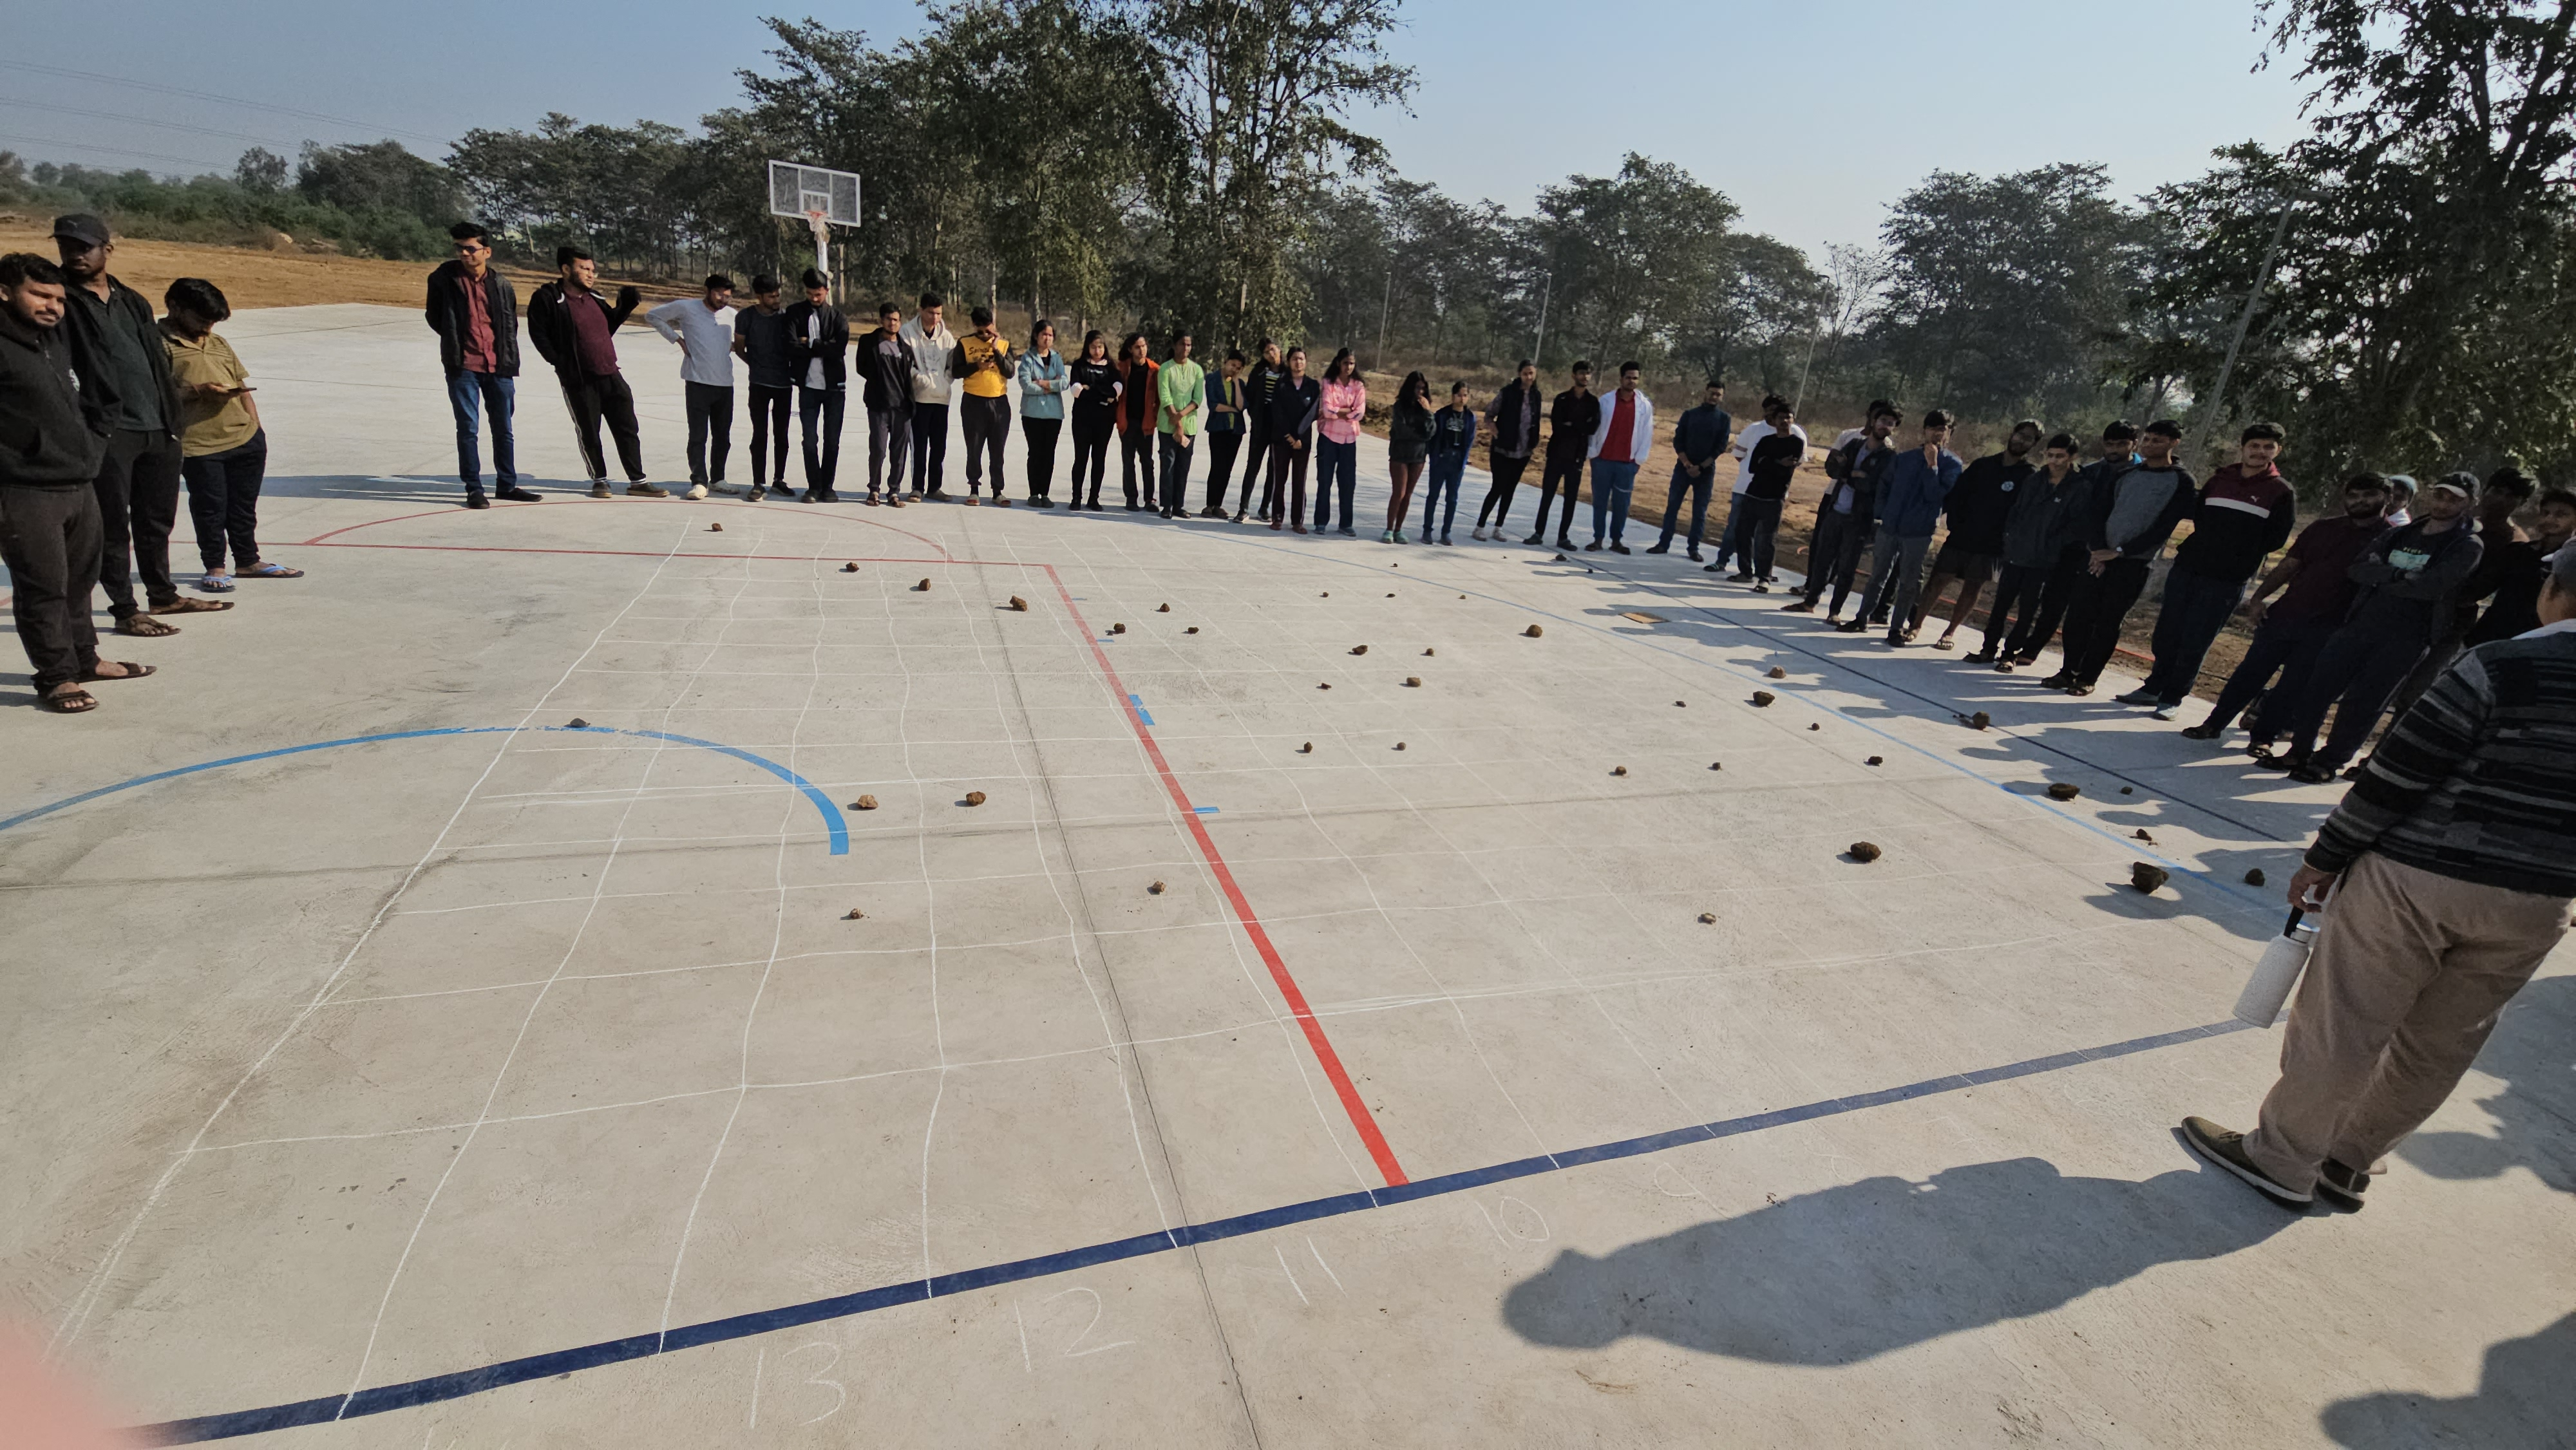
\includegraphics[width=0.7\linewidth]{VECTOR.jpg}
    \caption{VECTOR}
    \label{fig:VECTOR}
\end{figure}




---

Part 3: \textit{Python Implementation}


Let's implement the solution in Python using numpy to handle vector operations efficiently.

Python:-


import numpy as np


# Define the force vectors \ 

F1 = np.array([10, 5])  # Force from person 1 \ 

F2 = np.array([-8, 7])  # Force from person 2 \ 

F3 = np.array([3, -6])  # Force from person 3 \ 


Step 1: Calculate the net force (vector sum)
net_force = F1 + F2 + F3

Step 2: Calculate the magnitude of the net force
magnitude = np.linalg.norm(net_force)

Step 3: Find the direction of the net force (angle with respect to x-axis) \ 

direction = np.arctan2(net_force[1], net_force[0])  Angle in radians \ 

direction_degrees = np.degrees(direction)  # Convert to degrees \  


%Display the results
print("Net Force Vector (F_net):", net_force)

print("Magnitude of Net Force:", magnitude, "Newtons")

print("Direction of Net Force:", direction_degrees, "degrees") 


\setlength{\parskip}{1em}


---
\ 
 \ 
  \

   
\textbf{Output:}




Net Force Vector (F_net): [5 6]

Magnitude of Net Force: 7.810249675906654 Newtons

Direction of Net Force: 50.19442890773457 degrees. 




\textbf{Click here to watch the video: }\href{https://drive.google.com/file/d/1VlTeJLOTASAtO9nbkH_QxsGp8jWv7EO0/view?usp=drive_link}{Watch Video}

\textbf{Click here to watch the video: }\href{https://drive.google.com/file/d/1Rbj_JCdAgs84ctgMNpFsYSufM_-e7lto/view?usp=drive_link}{Watch Video} 


\textbf{Click here to watch the video: }\href{https://drive.google.com/file/d/10KBo4J0sRjEIQccBlL08HJFJY9zLl3Rw/view?usp=drive_link}{Watch Video} 





\setlength{\parskip}{1em}
\ 
 \ 
 \ 
 \  
 \ 
   \ 
   \ 
   \ 
\paragraph{   }
   \textbf{CONDITIONAL PROBABILITY:-}



Conditional probability is the probability of an event occurring given that another event has already occurred. In other words, it quantifies the likelihood of an event \( A \) happening, under the condition that event \( B \) is known to have occurred. The conditional probability of \( A \) given \( B \) is denoted as \( P(A | B) \), and it is calculated using the formula:


\[
P(A | B) = \frac{P(A \cap B)}{P(B)}
\]

\textit{where:}

- \( P(A \cap B) \) is the probability that both events \( A \) and \( B \) occur (i.e., the intersection of \( A \) and \( B \)).
- \( P(B) \) is the probability that event \( B \) occurs.



### \textbf{Dice Experiment and Conditional Probability}




Let's consider a dice experiment. We roll a standard 6-sided die, and let’s define the following events:


- *Event A*: The die shows an even number (2, 4, or 6).

- *Event B*: The die shows a number greater than 3 (4, 5, or 6).

We want to calculate the conditional probability of event A given that event B has occurred, i.e., \( P(A | B) \).

### \textit{Step-by-Step Calculation}:-


#### Step 1: Define the Sample Space
The sample space \( S \) for a 6-sided die is:

\[
S = \{1, 2, 3, 4, 5, 6\}
\]

#### Step 2: Calculate the Probability of Event B, \( P(B) \)
Event B occurs when the die shows a number greater than 3. So, \( B = \{4, 5, 6\} \). The probability of event B is:

\[
P(B) = \frac{\text{Number of outcomes in } B}{\text{Total number of outcomes in } S} = \frac{3}{6} = 0.5
\]

#### Step 3: Calculate the Probability of the Intersection of Events A and B, \( P(A \cap B) \)
The intersection of events A and B, \( A \cap B \), occurs when the die shows a number that is both even (from event A) and greater than 3 (from event B). The numbers that satisfy both conditions are \( \{4, 6\} \).

So, \( A \cap B = \{4, 6\} \), and the probability of this intersection is:

\[
P(A \cap B) = \frac{\text{Number  of  outcomes  in  } A \cap B}{\text{Total number  of  outcomes  in }  S} = \frac{2}{6} = 0.3333
\]

#### Step 4: Apply the Conditional Probability Formula
Now, we can apply the formula for conditional probability:

\[
P(A | B) = \frac{P(A \cap B)}{P(B)} = \frac{\frac{2}{6}}{\frac{3}{6}} = \frac{2}{3}
\]

So, the conditional probability of event A (the die shows an even number) given that event B (the die shows a number greater than 3) has occurred is:

\[
P(A | B) = \frac{2}{3}
\]

\setlength{\parskip}{1em}
\ 

###\textit{ Interpretation} 


Given that the die has shown a number greater than 3, the probability that it is also an even number (either 4 or 6) is \( \frac{2}{3} \). This conditional probability helps us understand how the knowledge of event B influences the likelihood of event A.



%\documentclass{article}
%\usepackage{amsmath}
%\usepackage{booktabs} % For nicer tables
%\usepackage{geometry} % For adjusting margins
%\geometry{margin=1in}

\begin{document}

\section*{Activity: Understanding Conditional Probability Using a Dice Experiment}

\subsection*{Objective}
To understand the concept of conditional probability through a simple dice-rolling experiment.

\subsection*{Materials Needed}
\begin{itemize}
    \item A six-sided die (standard die with faces numbered 1 to 6).
    \item Pen and paper (or a whiteboard) for recording outcomes.
\end{itemize}

\subsection*{Instructions}

\subsubsection*{Step 1: Define the Experiment}
\begin{enumerate}
    \item Roll a standard six-sided die multiple times (e.g., 20 trials).
    \item Record the outcome of each roll.
\end{enumerate}

\subsubsection*{Step 2: Define Events}
Let:
\begin{itemize}
    \item \textbf{Event A}: The die roll results in an even number (\(\{2, 4, 6\}\)).
    \item \textbf{Event B}: The die roll results in a number greater than 3 (\(\{4, 5, 6\}\)).
\end{itemize}

\subsubsection*{Step 3: Conduct the Experiment}
\begin{enumerate}
    \item Roll the die and record the outcomes.
    \item For each roll, determine whether it satisfies Event A, Event B, or both.
\end{enumerate}

\subsubsection*{Step 4: Analyze the Results}
\begin{enumerate}
    \item Count the number of rolls where:
          \begin{itemize}
              \item Event A occurs (\( n(A) \)).
              \item Event B occurs (\( n(B) \)).
              \item Both Event A and Event B occur (\( n(A \cap B) \)).
          \end{itemize}
    \item Use the frequency of these events to estimate probabilities:
          \[
          P(A) = \frac{n(A)}{\text{total rolls}}, \quad 
          P(B) = \frac{n(B)}{\text{total rolls}}, \quad 
          P(A \cap B) = \frac{n(A \cap B)}{\text{total rolls}}.
          \]
\end{enumerate}

\subsubsection*{Step 5: Calculate Conditional Probabilities}
Using the formula for conditional probability:
\[
P(A \mid B) = \frac{P(A \cap B)}{P(B)}
\]
\begin{enumerate}
    \item Substitute the experimental values of \( P(A \cap B) \) and \( P(B) \) into the formula.
    \item Interpret the result:
          \begin{itemize}
              \item \( P(A \mid B) \): Probability of rolling an even number, given that the number is greater than 3.
          \end{itemize}
\end{enumerate}

\subsection*{Example of Recorded Data (Sample Table)}

\begin{center}
\begin{tabular}{cccccc}
\toprule
\textbf{Trial} & \textbf{Outcome} & \textbf{Event A (Even)} & \textbf{Event B (\(>3\))} & \textbf{Both A and B} \\ 
\midrule
1 & 4 & Yes & Yes & Yes \\ 
2 & 2 & Yes & No & No \\ 
3 & 5 & No & Yes & No \\ 
4 & 6 & Yes & Yes & Yes \\ 
5 & 3 & No & No & No \\ 
\midrule
... & ... & ... & ... & ... \\ 
\bottomrule
\end{tabular}
\end{center}

\subsection*{Discussion Points}
\begin{enumerate}
    \item \textbf{Theoretical Probability}:
          \begin{itemize}
              \item \( P(A) = \frac{3}{6} = 0.5 \) (since there are 3 even numbers out of 6).
              \item \( P(B) = \frac{3}{6} = 0.5 \) (since there are 3 numbers greater than 3).
              \item \( P(A \cap B) = \frac{2}{6} = 0.333 \) (only 4 and 6 satisfy both conditions).
          \end{itemize}
          Using these values:
          \[
          P(A \mid B) = \frac{P(A \cap B)}{P(B)} = \frac{0.333}{0.5} \approx 0.666
          \]
    \item \textbf{Connection to Real-World Applications}:
          Conditional probability is used in fields like medicine (e.g., probability of disease given a positive test result) and weather forecasting.
\end{enumerate}

\subsection*{Extension Activity}
\begin{itemize}
    \item Modify the conditions of the experiment. For example:
          \begin{itemize}
              \item Event A: Rolling a multiple of 3 (\(\{3, 6\}\)).
              \item Event B: Rolling an odd number (\(\{1, 3, 5\}\)).
          \end{itemize}
    \item Explore the relationship between the events when they are independent or mutually exclusive.
\end{itemize}





\textit{\textbf{Python Code Implementation:-}}

We can simulate this dice experiment and compute the conditional probability using Python:




import numpy as np


# Define the sample space for a 6-sided die

sample_space = [1, 2, 3, 4, 5, 6]


# Define the events A and B

A = [2, 4, 6]  # Even numbers

B = [4, 5, 6]  # Numbers greater than 3


# Calculate P(A ∩ B) - intersection of A and B

intersection_A_B = list(set(A) & set(B))


# Calculate P(B)

P_B = len(B) / len(sample_space)


# Calculate P(A ∩ B)


P_A_intersection_B = len(intersection_A_B) / len(sample_space)



# Calculate P(A | B) using the formula


P_A_given_B = P_A_intersection_B / P_B



# Display the result


print("P(A | B) =", P_A_given_B)




### Output:


text

P(A | B) = 0.6666666666666666



This Python code confirms our theoretical calculation that the conditional probability of event A given event B is \( \frac{2}{3} \). 




\textbf{Click here to watch the video: }\href{https://drive.google.com/file/d/1w9gS_nut-K0EZZ5SGK8UsKN_qbwcPaBN/view?usp=drive_link}{Watch Video} 

\textbf{Click here to watch the video: }\href{https://drive.google.com/file/d/1RaYIik78RKVCLtHUbQN0TbpetEXeckl6/view?usp=drive_link}{Watch Video} 

\textbf{Click here to watch the video: }\href{https://drive.google.com/file/d/1J6ZlfSrlUJupLeQZTIPitkgY0OLLZeeK/view?usp=drive_link}{Watch Video} 




\end{document}
